\subsection{Setup initial}

Toute cette partie est couverte par la formation précédente. Normalement, à la suite de tutoriel, vous devriez avoir obtenu le site suivant en vous rendant sur \url{http://lurlquevousavezchoisie}:\footnote{\underline{PS:}n'oubliez pas de lancer \verb|sail up -d| et \verb|sail npm run dev| si cela n'est pas déjà fait! Ne vous inquiétez pas, l'explication pour la deuxième commande va bientôt arriver\ldots}.
\begin{figure}[!h]
    \centering
    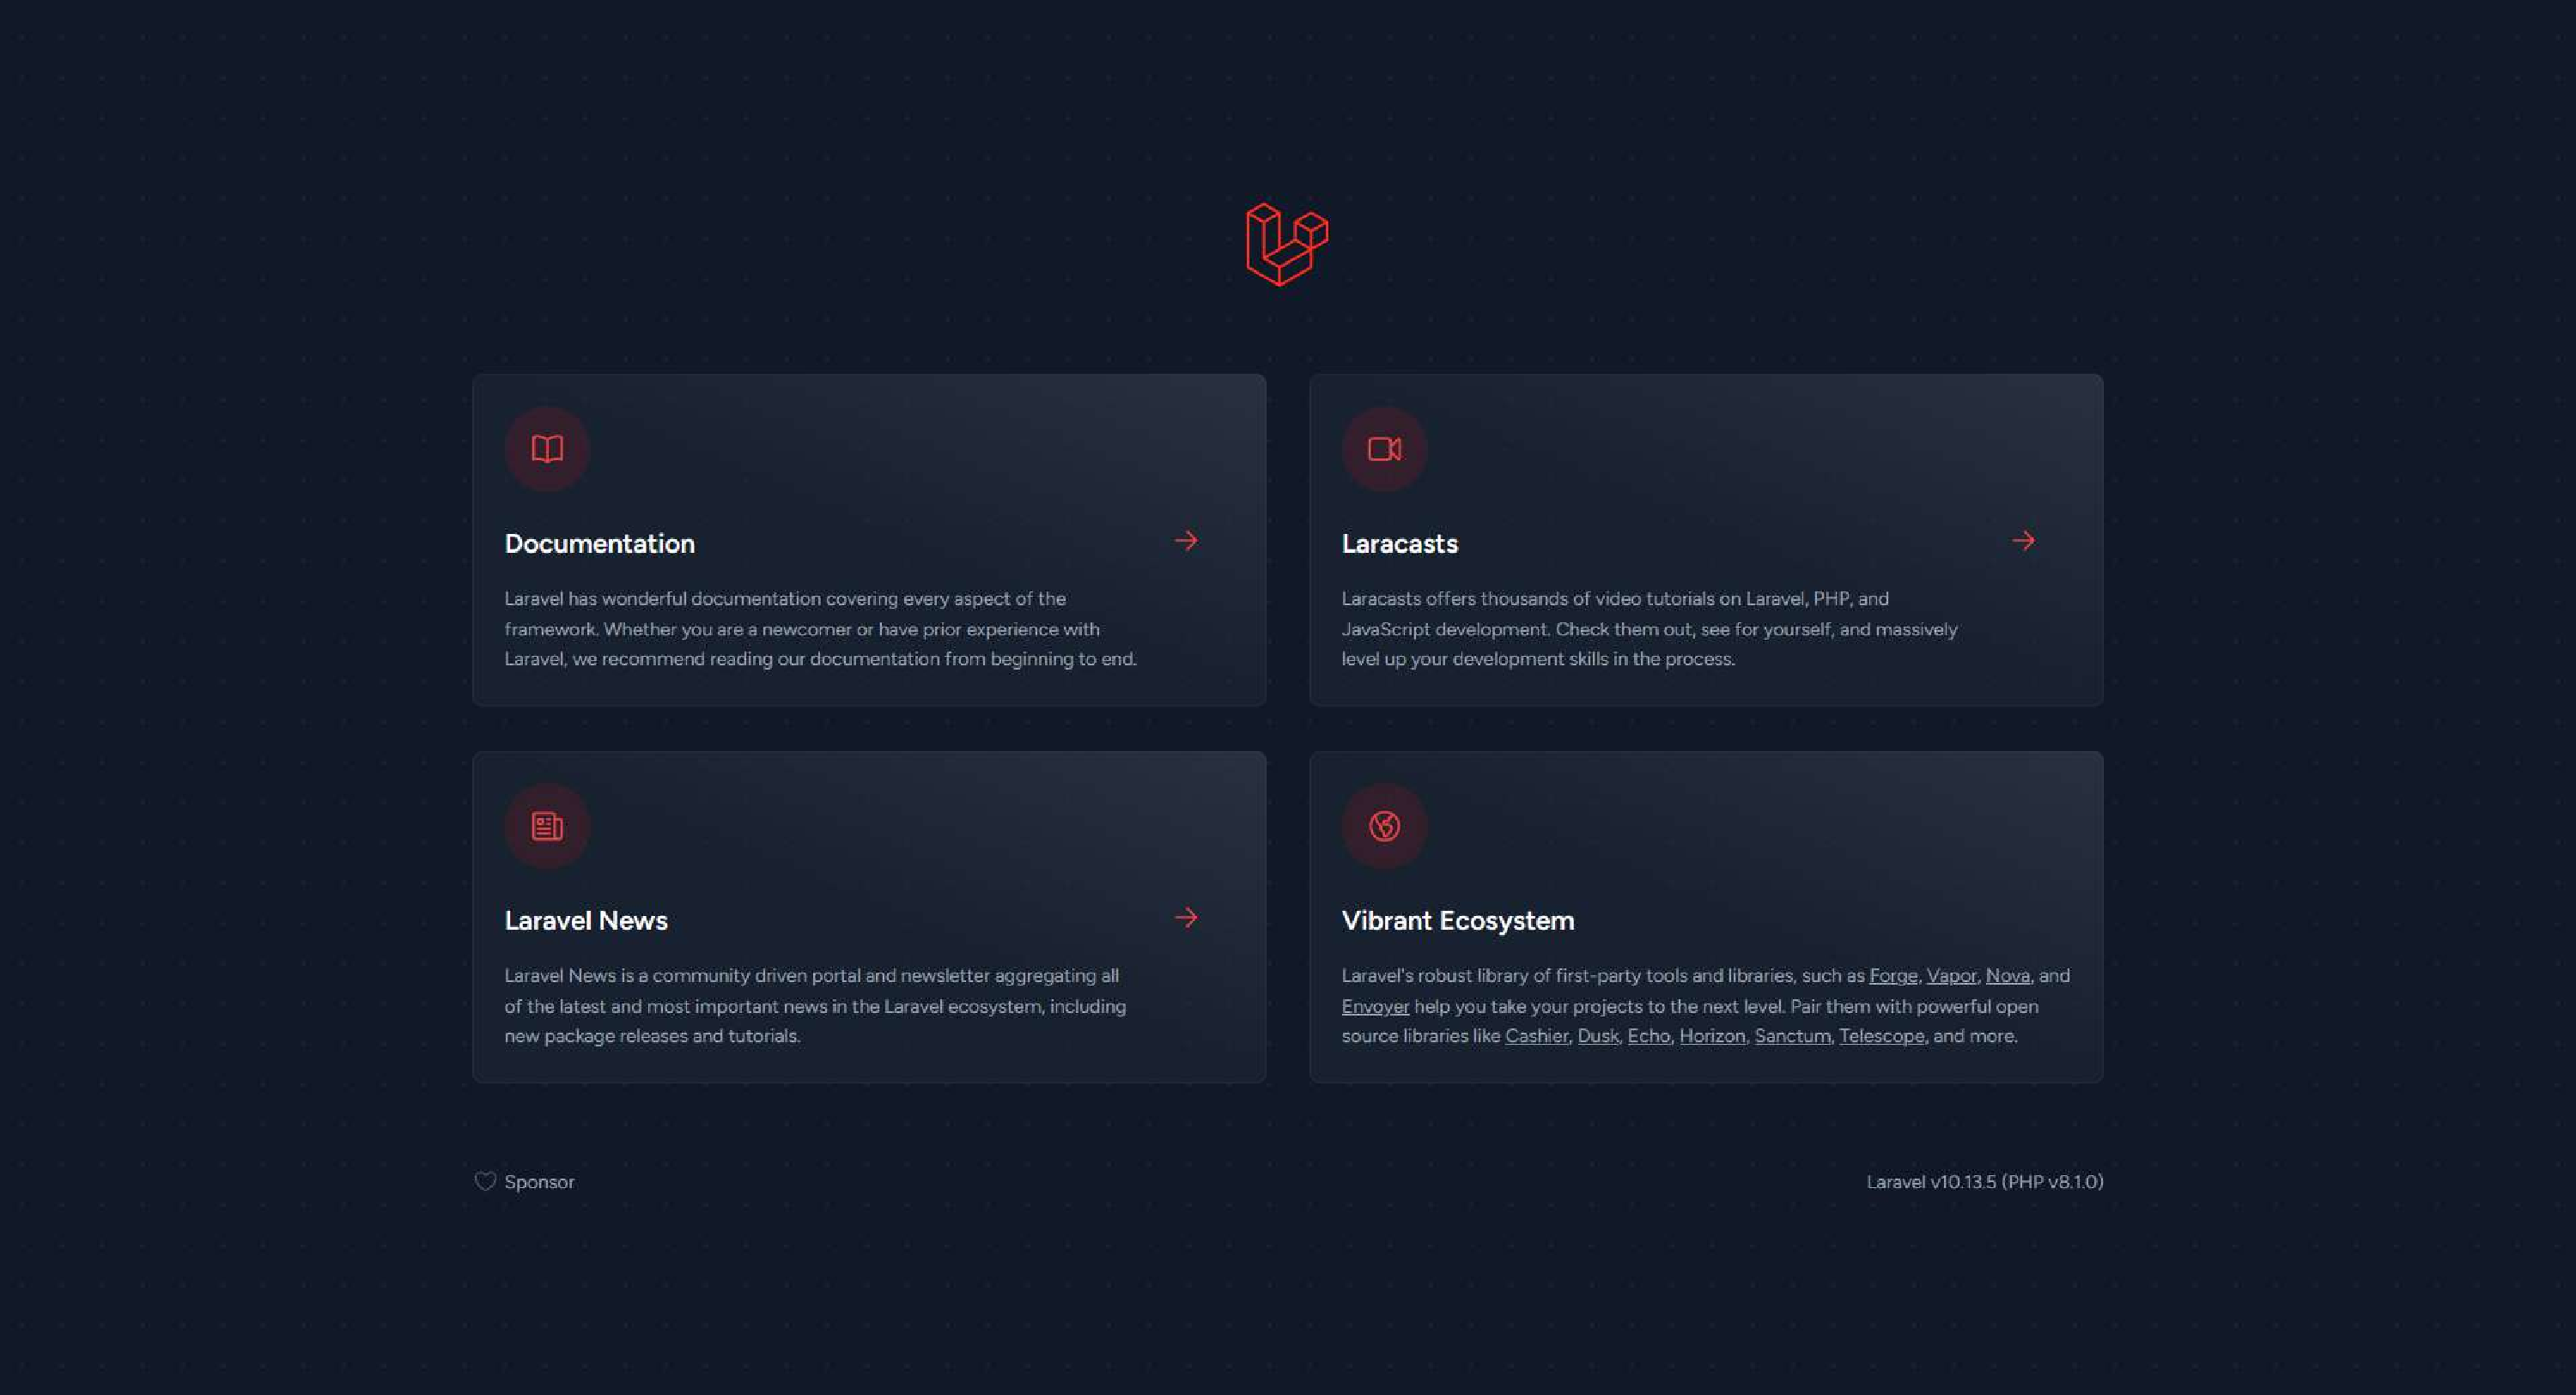
\includegraphics[width=0.75\textwidth]{figures-C1/laravel_default_website.pdf}
\end{figure}
Nous allons partir de ce site là. Pour ce tutoriel, mon projet sera appellé \texttt{tutorialstepbystep} donc son URL sera \url{http://tutorialstepbystep/}.
